

\section{Experimental setup}
\label{sec:experiment}

The analysis is performed with data samples in pp collisions at $\sqrt{s} = 13$~TeV collected from 2016 to 2018 and in p--Pb collisions at $\sqrt{s_\mathrm{NN}} = 5.02$~TeV in 2016 during the LHC Run 2 period. A full description of the ALICE detector and performance in the LHC Run 2 can be found in Refs~\cite{Aamodt:2008zz,Abelev:2014ffa}. The analysis utilizes the V0 detector~\cite{Abbas:2013taa}, the Inner Tracking System (ITS)~\cite{aliceITS}, and the Time Projection Chamber (TPC)~\cite{aliceTPC}. 

The V0 detector consists of two stations on both sides of the interaction point, V0A and V0C, each made of 32 plastic scintillator tiles, covering the full azimuthal angle within the pseudorapidity intervals $2.8 < \eta < 5.1$ and $-3.7 < \eta < -1.7$, respectively. The V0 provides a minimum-bias (MB) trigger in both pp and p--Pb collisions and an additional high-multiplicity trigger in pp collisions. The minimum bias trigger is obtained by a time coincidence of V0A and V0C signals. The charged particle multiplicity is determined based on the sum of the V0A and V0C signals, which is denoted as V0M. The high-multiplicity trigger requires the V0M signal to exceed 5 times the mean value measured in MB collisions, selecting the 0.1\% of MB events with the largest V0M multiplicity. The analyzed data samples of MB and high-multiplicity pp events at $\sqrt{s}=$~13 TeV correspond to integrated luminosities ($\mathcal{L}_\mathrm{int}$) of 19 nb$^{-1}$ and 11 pb$^{-1}$, respectively~\cite{ALICE-PUBLIC-2016-002}. In p--Pb collisions at $\sqrt{s_\mathrm{NN}} = 5.02$ TeV, the number of events corresponding to $\mathcal{L}_\mathrm{int} = 3$ nb$^{-1}$ is used for the analysis. 

The primary vertex positions are reconstructed from signals measured by the Silicon Pixel Detector (SPD)~\cite{Santoro2009:ALICESPD}, consisting of the two innermost layers of the ITS. The reconstructed primary vertices are required to be within 8 cm of the nominal interaction point along the beam direction. Pileup events are determined and rejected if the longitudinal displacement of the secondary vertex is greater than 0.8 cm in pp collisions. The probability of pileup events is estimated to be about 0.6\% for MB and high-multiplicity events in pp collisions. The pileup probability is estimated to be negligible in p--Pb collisions. 

Charged-particle tracks are reconstructed using the combined information of the ITS and TPC in a uniform magnetic field of 0.5 T along the beam direction by the solenoid. The ITS is a silicon tracker with six layers of silicon sensors; the SPD consists of the two innermost layers, the next two layers are the SDD (Silicon Drift Detector), and the outermost layers are the SSD (Silicon Strip Detector). The ITS and TPC cover the entire azimuth range up to $|\eta|<1.4$ and 0.9, respectively, for detecting charged particles emitted within 8 cm from the nominal vertex position $z_\mathrm{vtx}=0$ along the beam direction. Charged particle tracking is performed with the ITS and TPC capable of reconstructing tracks down to transverse momentum ($\pt$) of 0.15 GeV/$c$ with an efficiency of about 65\% and the efficiency reaches 80\% for intermediate $\pt$, 1--5~GeV/$c$. The $\pt$ resolution is about 1\% (1\%) for primary charged particles with $\pt<$~1~GeV/$c$, linearly increasing to 6\% (10\%) at $\pt\sim$ 50~GeV/$c$ in pp (p--Pb) collisions~\cite{ALICE:2018vuu}. 

The charged particle selection criteria are optimized to ensure a uniform efficiency over the sensitive TPC volume to mitigate the effects of small areas where some ITS layers are inactive in both collision systems. The selection consists of two classes of tracks. Those in the first class must have at least one hit in SPD. The tracks of the second class do not have any hits related to the SPD, and their origins are rather constrained to the primary vertex~\cite{ALICE:2012eyl}. 

\section{Analysis procedure}
\label{sec:ana}
\subsection{Two-particle angular correlations}
Two-particle angular correlations are measured as functions of the relative azimuthal angle ($\Delta\varphi$) and the relative pseudorapidity ($\Delta\eta$) between a trigger and associated particles
\begin{eqnarray}
\frac{1}{N_{\rm{trig}}} \frac{ \rm{d}\it{}^{2} N_{\rm{pair}} }{ \rm{d} \Delta\eta \rm{d}\Delta\varphi} = B(0, 0)\frac{S(\Delta\eta, \Delta\varphi)}{B(\Delta\eta, \Delta\varphi)}  \Big\lvert_{\pttrig,\,\ptassoc}\quad , 
\label{eq:corrfunction}
\end{eqnarray}
where the transverse momentum range for associated particles ($p_\mathrm{T,assoc}$) is $1<p_\mathrm{T,assoc}<4$~GeV/$c$ for different transverse momentum ranges of trigger particles ($p_\mathrm{T,trig}$).
The $N_\mathrm{trig}$ and $N_\mathrm{pair}$ are the numbers of trigger particles and trigger-associated particle pairs, respectively. $S(\Delta\eta, \Delta\varphi)$ corresponds to the average number of pairs in the same event and $B(\Delta\eta, \Delta\varphi)$ to the number of pairs in mixed events. 
$B (0,0)$ represents the normalization of $B(\Delta\eta, \Delta\varphi)$, and by dividing $S(\Delta\eta, \Delta\varphi)$ with $B(\Delta\eta, \Delta\varphi)/B (0,0)$ the acceptance effects are corrected for. The particles are corrected by weighting with the inverse of the tracking efficiency, obtained in the same way as in the previous study in Ref.~\cite{ALICE:2021nir}.
%The tracking inefficiency is corrected for on the right-hand side of Eq.~\ref{eq:corrfunction} as functions of $p_\mathrm{T}$ and $\eta$. 
In the previous study~\cite{ALICE:2021nir}, the tracking efficiency was calculated with a detector simulation with the PYTHIA 8 event generator and the GEANT3 transport code~\cite{Brun:1994aa}. The tracking efficiency is determined by re-weighting the primary particle composition based on a data-driven method~\cite{ALICE:2018hza,ALICE:2018vuu}. 
%Therefore, this method improves the jet-yield extraction and has no impact on the flow extraction.
The pairs in mixed events are required to have primary vertices within the same 2 cm wide $z_{vtx}$ interval, and the correlation functions are averaged over the vertex bins, resulting in the final per-trigger yield~\cite{KOPYLOV1974472:evtmixing,Adam:2016tsv}. The lower limit of $p_\mathrm{T,trig}$ and $p_\mathrm{T,assoc}$ ($> 1~GeV$/$c$) is chosen in order to avoid jet-like contributions which extend into the larger $\Delta\eta$ range for lower $p_\mathrm{T}$ particles because of the limited $\eta$ acceptance~\cite{ALICE:2021nir} . 

\begin{figure}[h!]
		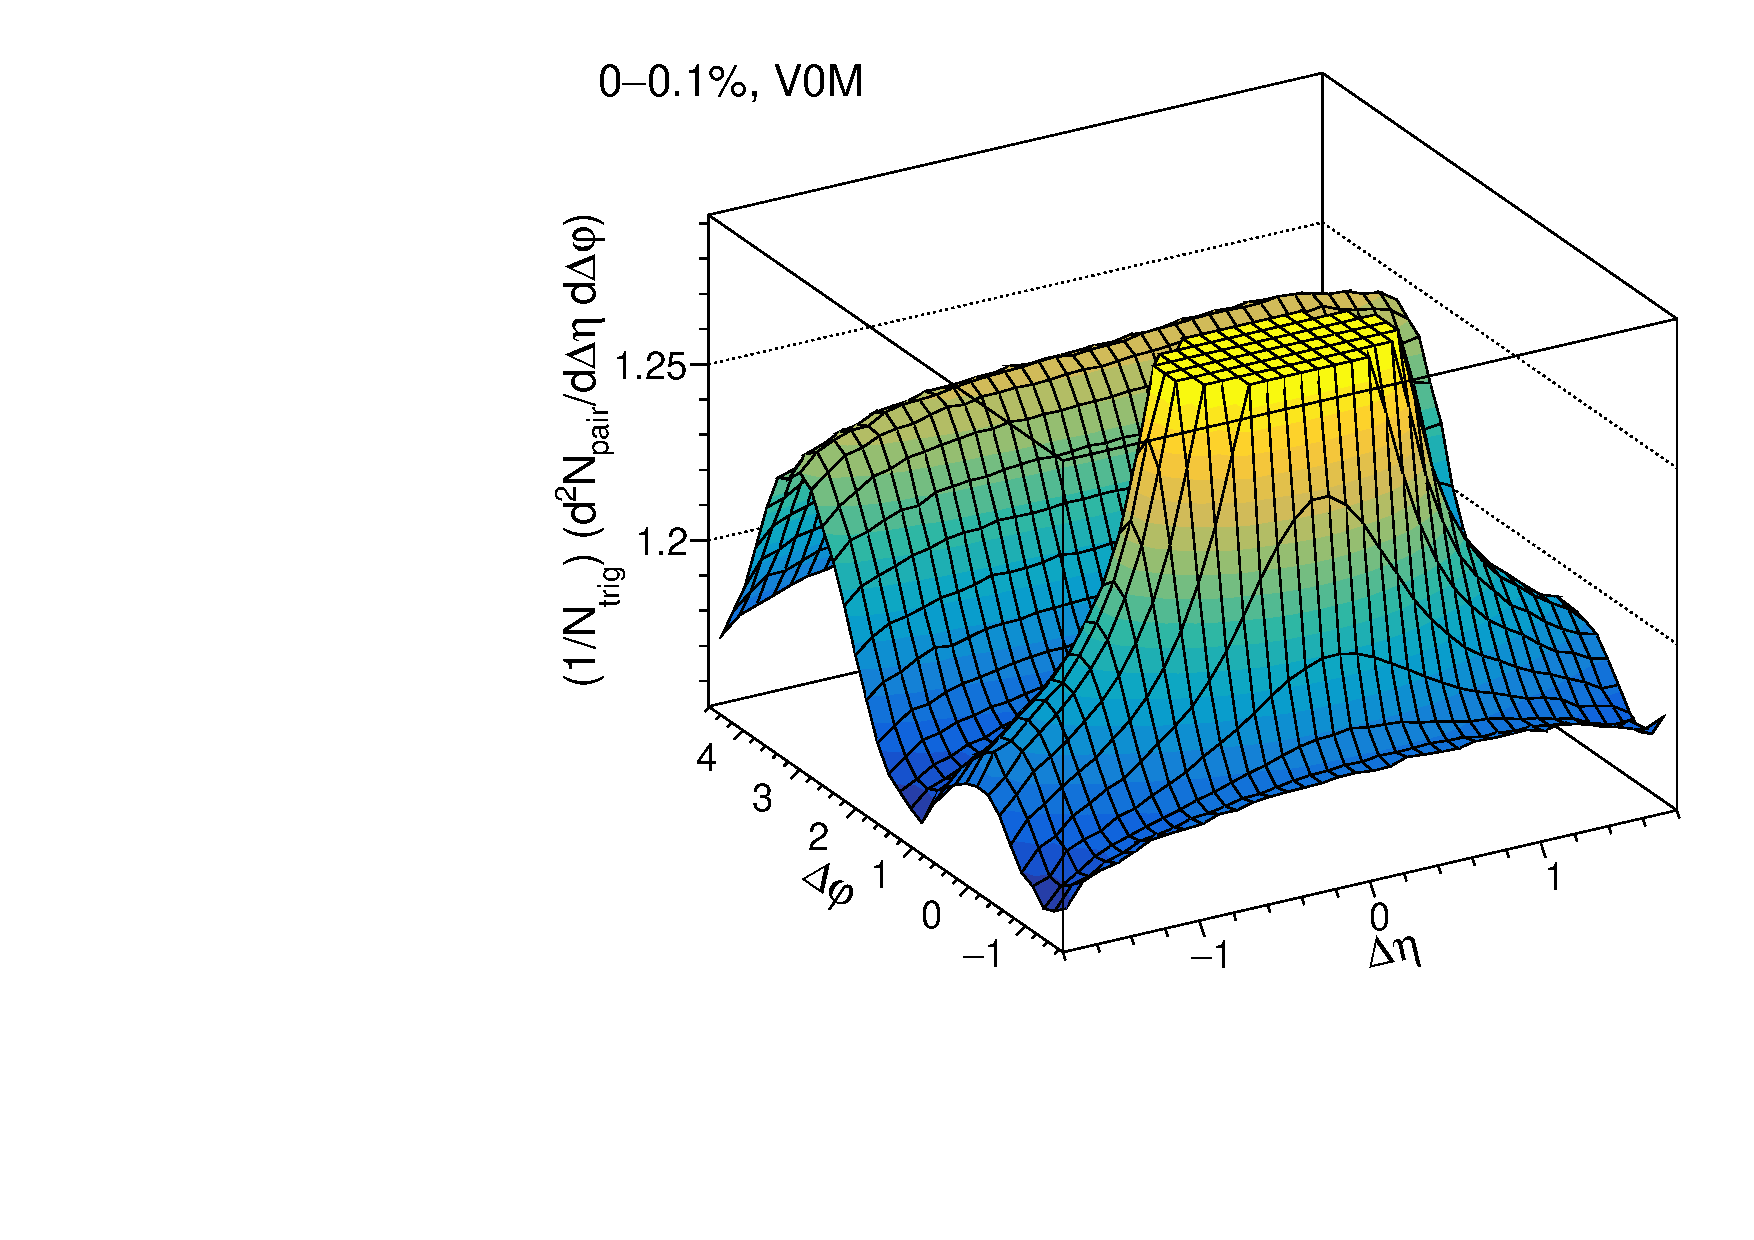
\includegraphics[width=0.5 \textwidth]{figures/Fig1_ppHigh.pdf} 
		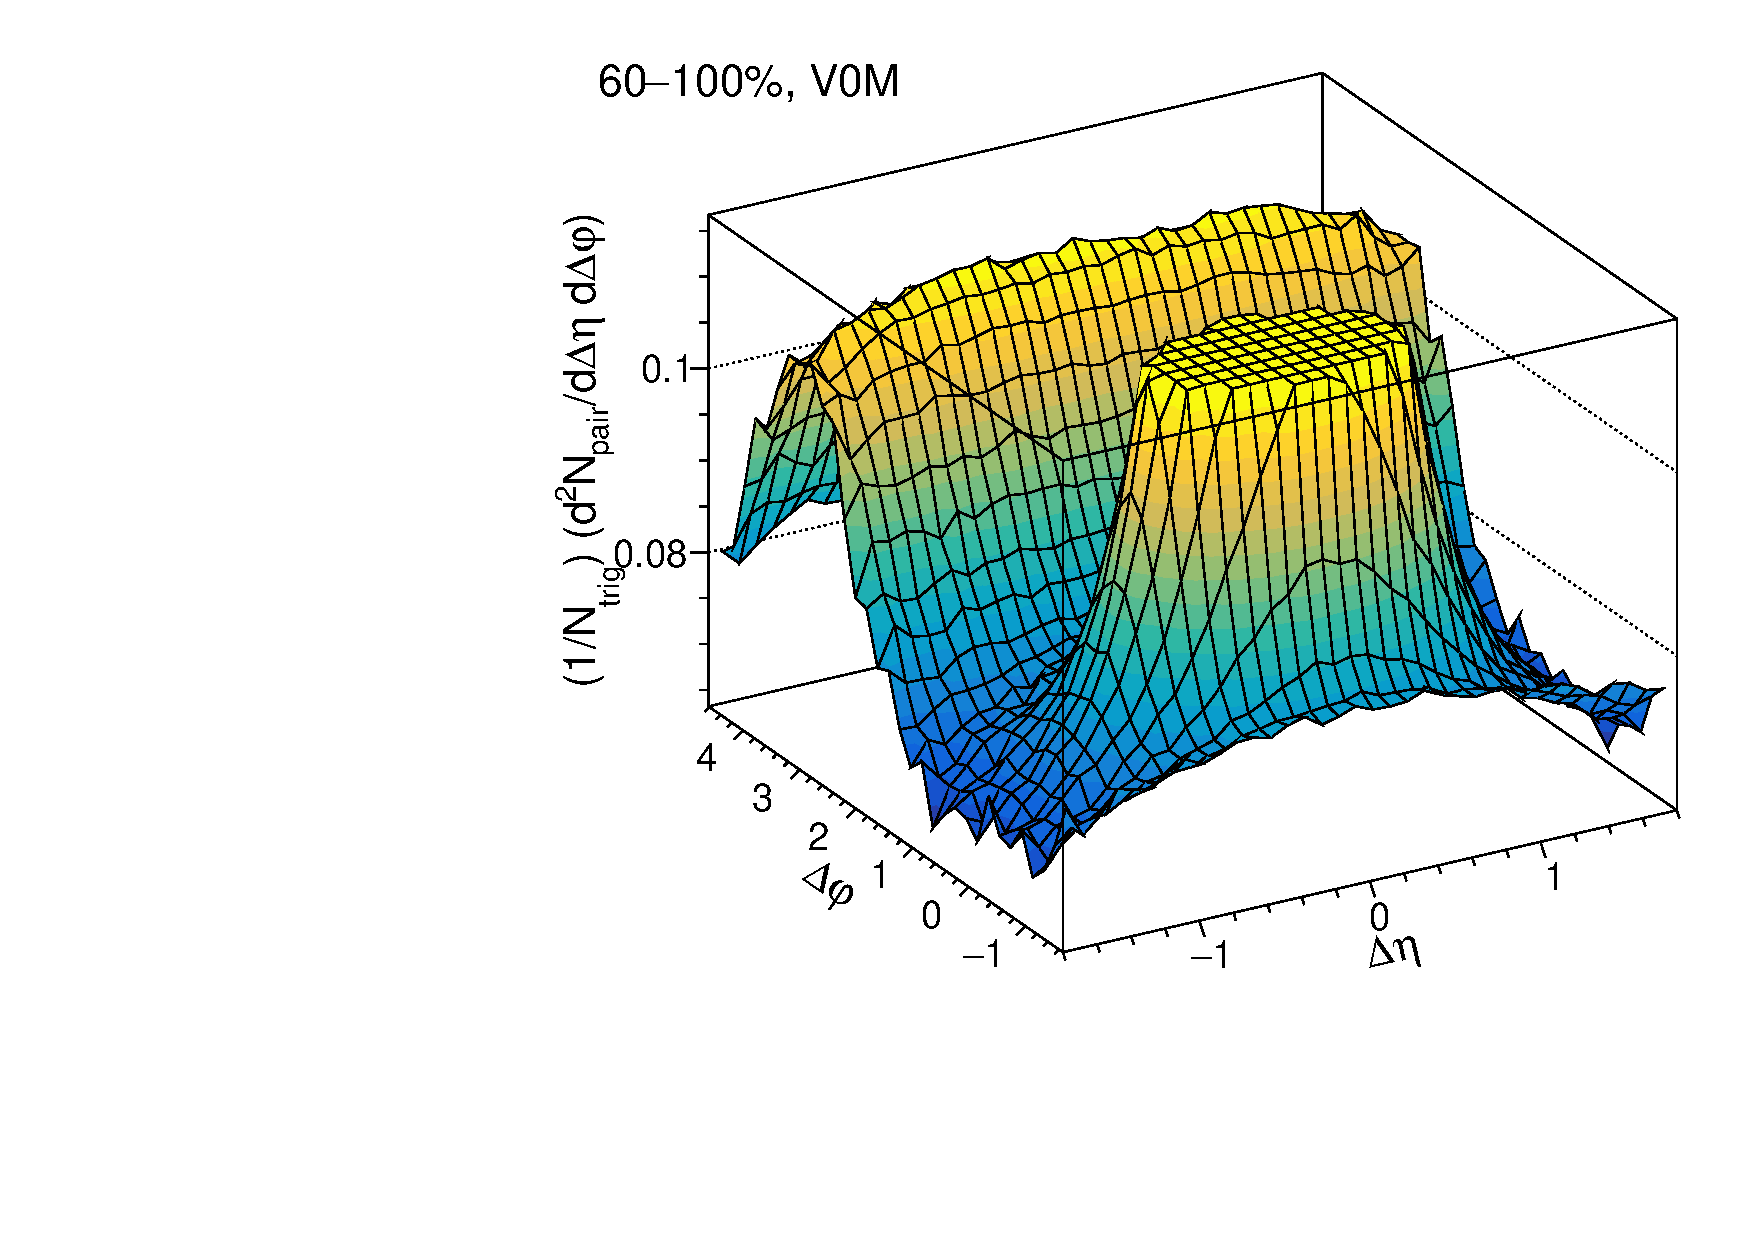
\includegraphics[width=0.5 \textwidth]{figures/Fig1_ppLow.pdf} 
  		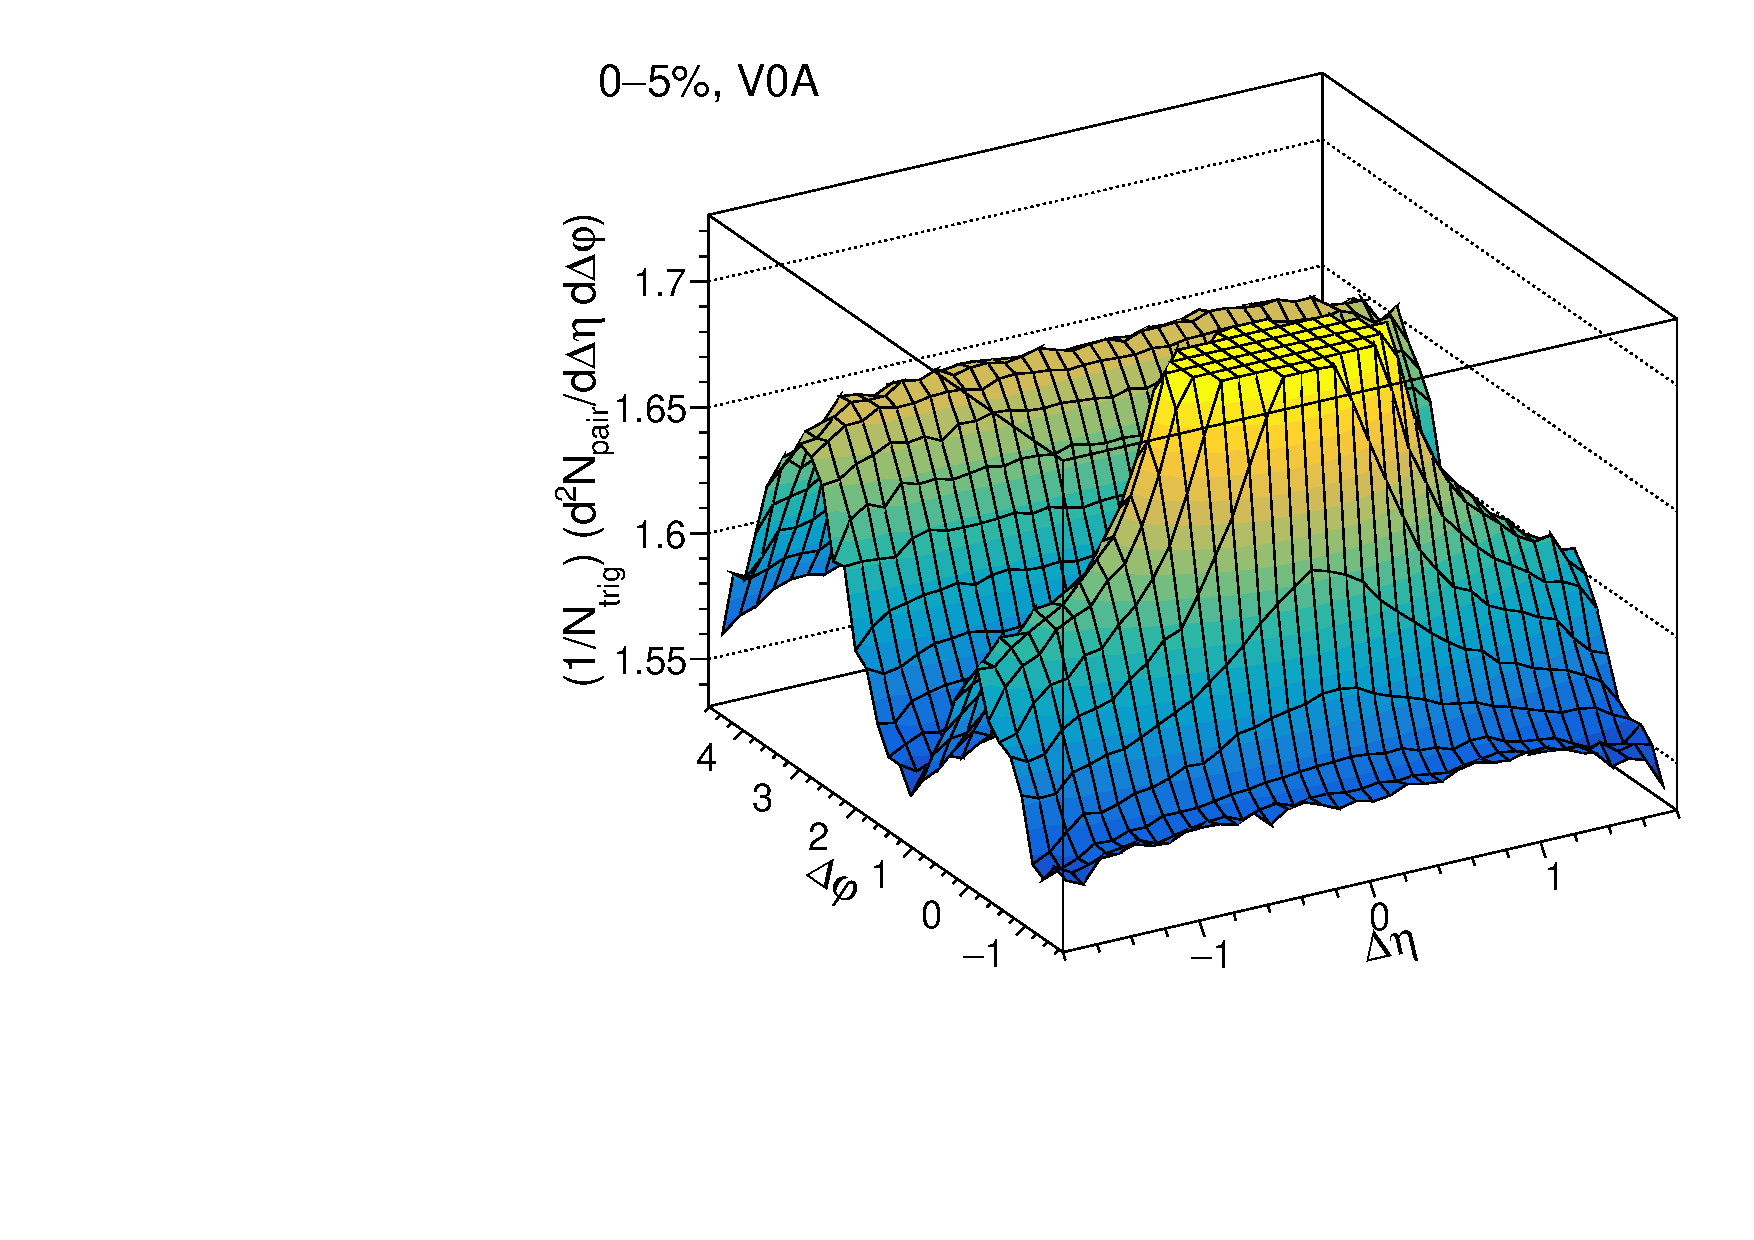
\includegraphics[width=0.5 \textwidth]{figures/Fig1_pPbHigh.pdf}
		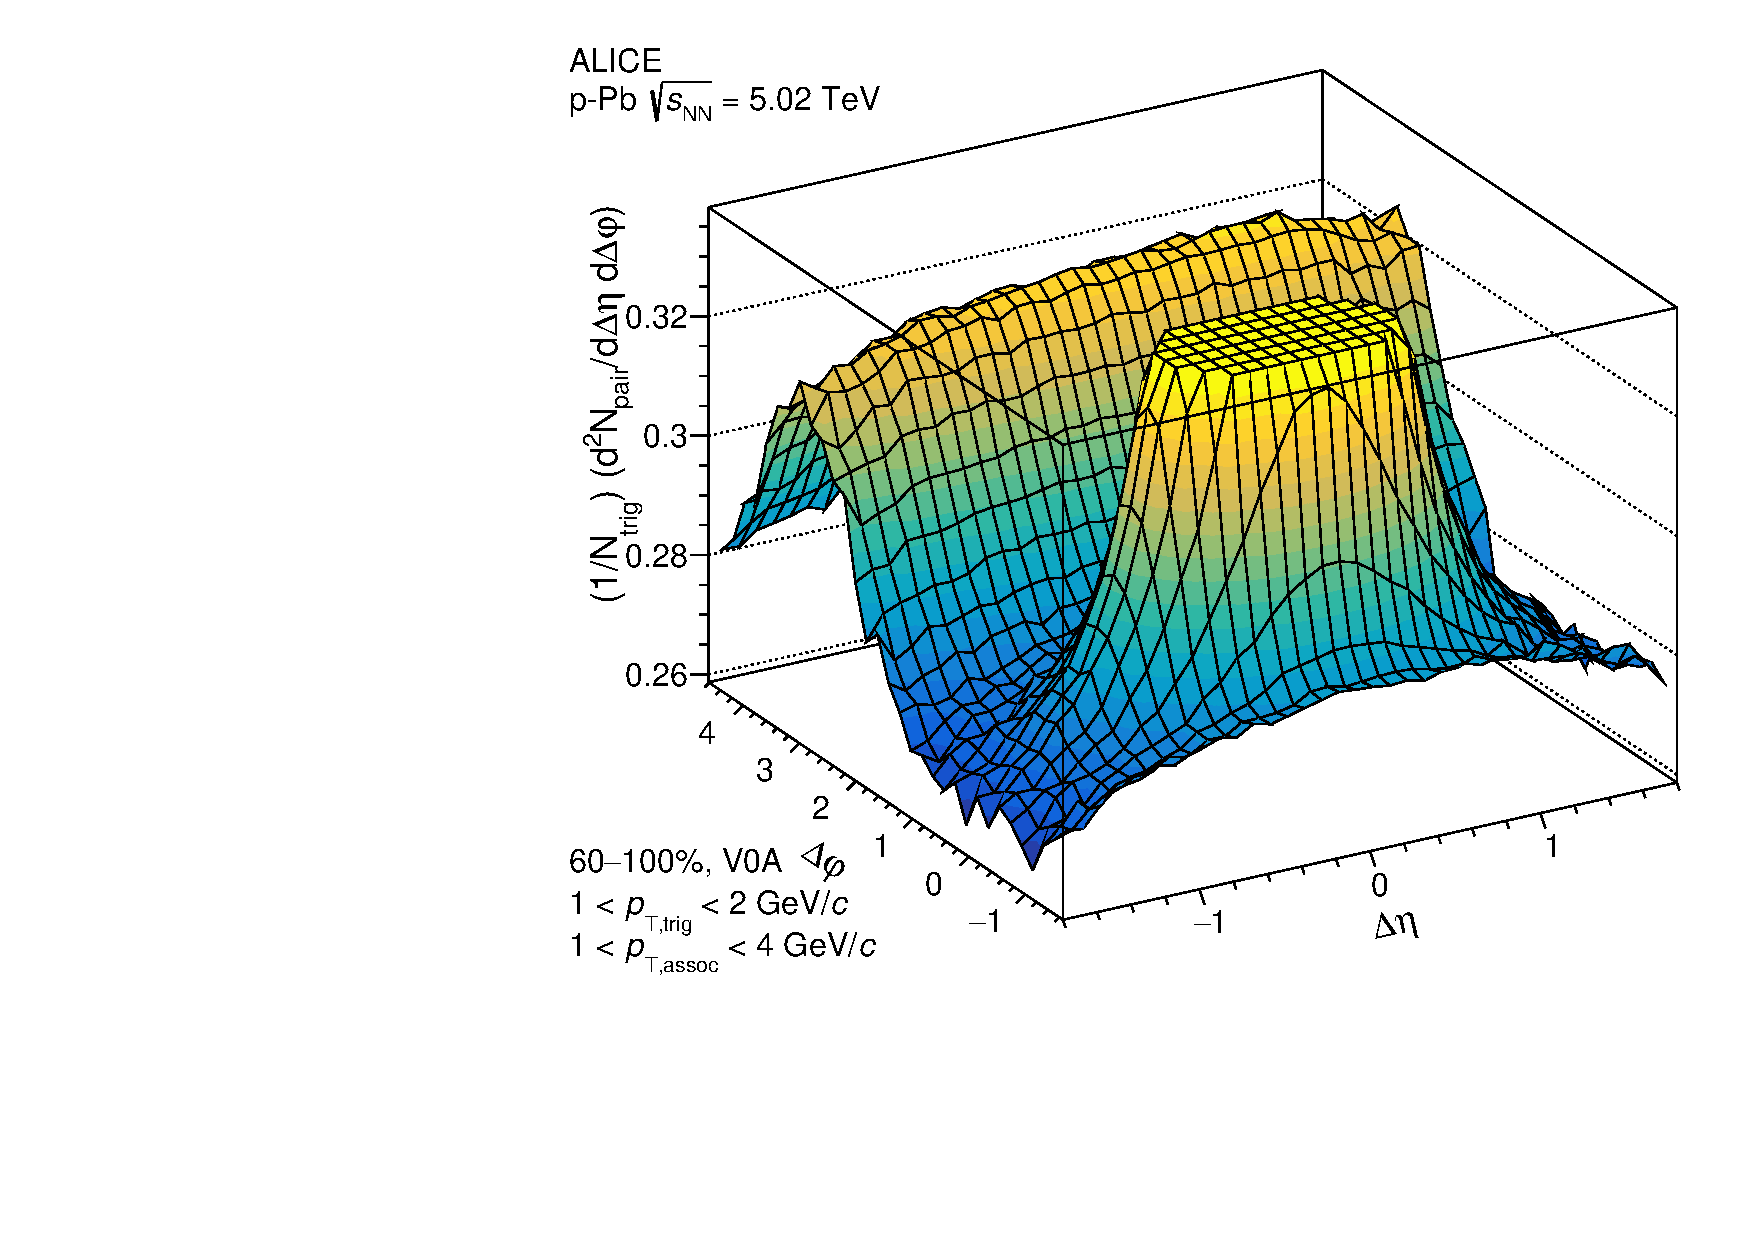
\includegraphics[width=0.5 \textwidth]{figures/Fig1_pPbLow.pdf}
\caption{The two-dimensional correlation functions as functions of $\Delta\eta$ and $\Delta\varphi$ are shown for high-multiplicity (0--0.1\% or 0--5\%, on the left) and low-multiplicity (60--100\%, on the right) events in $\sqrt{s}=13$ TeV pp collisions (top) and $\sqrt{s_{\mathrm{NN}}}=5.02$ TeV p--Pb collisions (bottom). The intervals of $\pttrig$ and $\ptassoc$ are 1~$<\it{p}_{\rm{T}}<$~2~GeV/$c$ in all cases.}
\label{fig:doubleridge}
\end{figure}

The two-dimensional correlation functions in pp collisions at $\sqrt{s}=13$ TeV are shown at the top panels in Fig.~\ref{fig:doubleridge} for the high-multiplicity (0--0.1\% for pp and 0--5\% for p--Pb, left) and low-multiplicity (60--100\% both for pp and p--pPb, right). The bottom panels show those in $\sqrt{s_{\mathrm{NN}}}=5.02$ TeV p--Pb collisions. 
%The multiplicity percentile of p--Pb collisions is wider as particle multiplicity, ranging from 0--5\%, compared to that of pp collisions.
%The $z$-axis for the correlation yield is properly scaled in order to zoom in the larger $\Delta\eta$ region.
The $z$-axis is scaled in order to resolve the structures in large $\Delta\eta$ regions.
As a result, the jet peaks are sheared off in both figures. The flow modulation structure is clearly observed in the high-multiplicity collisions for both systems, while it is not seen in the low-multiplicity collisions. The away-side regions are populated mostly by back-to-back jet correlations. 
%but they are reduced and compatible with the one in the near side in $|\Delta\eta| > 1.6$.



The per-trigger yield is extracted in multiplicity percentiles 0--0.1, 1--5, 5--20, 20--60, and 60--100\% in pp collisions (0--5, 5--10, 10--20, 20--40, 40--60, and 60--100\% in p--Pb collisions) in $\pt$ intervals at large $\Delta\eta$, at $1.6<|\Delta\eta|<1.8$ to remove the non-flow contributions from near-side jet fragments. The per-trigger yield as a function of $\Delta\varphi$ is expressed as
\begin{eqnarray}
Y(\Delta\varphi) = \frac{1}{N_{\rm{trig}}} \frac{ \rm{d}\it{}N_{\rm{pair}} }{ \rm{d}\Delta\varphi } = \int_{1.6<|\Delta \eta|<1.8} \left( \frac{1}{\it{N}_{\rm{trig}}} \frac{ \rm{d}\it{}^{2} N_{\rm{pair}} }{ \rm{d}\Delta\eta \rm{d}\Delta\varphi} \right) \dfrac{1}{\delta_{\Delta\eta}} \rm{d}\Delta \eta \quad ,
\label{eq:pertrigger}
\end{eqnarray}
where the factor $\delta_{\Delta\eta}=$~0.4 is used as a normalization to obtain the per trigger yield per unit of pseudorapidity.
%The Zero-Yield-At-Minimum (ZYAM) procedure~\cite{Ajitanand:2005jj} is the method used to subtract the baseline of the correlation. 


\subsection{Extraction of flow coefficients}

As discussed in Refs.\cite{ATLAS:2015hzw,ATLAS:2016yzd}, the correlation function in a given multiplicity percentile is fitted with 
\begin{eqnarray}
\label{eq:narray}
Y_{\rm{HM}}(\Delta\varphi) = G~(1 + 2v_{2,2}\cos(2\Delta\varphi) + 2v_{3,3}\cos(3\Delta\varphi)) + F~Y_{\rm{LM}}(\Delta\varphi) \quad,
\end{eqnarray}
where $Y_{\rm{LM}}(\Delta\varphi)$ is the low-multiplicity template and $Y_{\rm{HM}}(\Delta\varphi)$ is the higher multiplicity template relative to $Y_{\rm{LM}}(\Delta\varphi)$, G is the normalization factor for the Fourier component up to the third harmonic $v_{n,n}$. The scale factor $F$ corresponds to the relative away-side jet-like contribution with respect to the low-multiplicity template corresponding to the 60--100\% percentile~\cite{ALICE:2013tla,ALICE:2014mas}. 
The fit determines the scale factor $F$, pedestal $G$, and $v_{n,n}$ and is performed in various high-multiplicity classes as well as in different $p_\mathrm{T,trig}$ and $p_\mathrm{T,assoc}$ intervals. 
%This method does not rely on the zero yield at minimum (ZYAM) hypothesis~\cite{Ajitanand:2005jj} to subtract an assumed flat combinatorial component from the low-multiplicity template as done previously in Refs.~\cite{ATLAS:2012cix,ATLAS:2014qaj}. 
This method assumes that $Y_{\rm{LM}}$ does not contain a peak in the near side originating from jet fragmentation, and that the jet shape remains unchanged in high-multiplicity events compared to low-multiplicity events. The first assumption is well-verified using the selected low-multiplicity template. The second assumption, regarding the modification of jet shapes, was tested with projections of the near-side jet peaks on $\Delta\eta$, which do not show significant dependence on their shape on multiplicity~\cite{LAKOMOV2017329}. Additionally, the ATLAS Collaboration's study of high-multiplicity pp and p-Pb collisions in Ref.~\cite{ATLAS:2018ngv} provides further support for this assumption, as there is no evidence of jet quenching in these collisions~\cite{Adam:2014qja,Khachatryan:2016odn,Adam:2016jfp,Adam:2016dau,Acharya:2017okq}.

\begin{figure}[h!]
	\centering
	\hspace{-3em}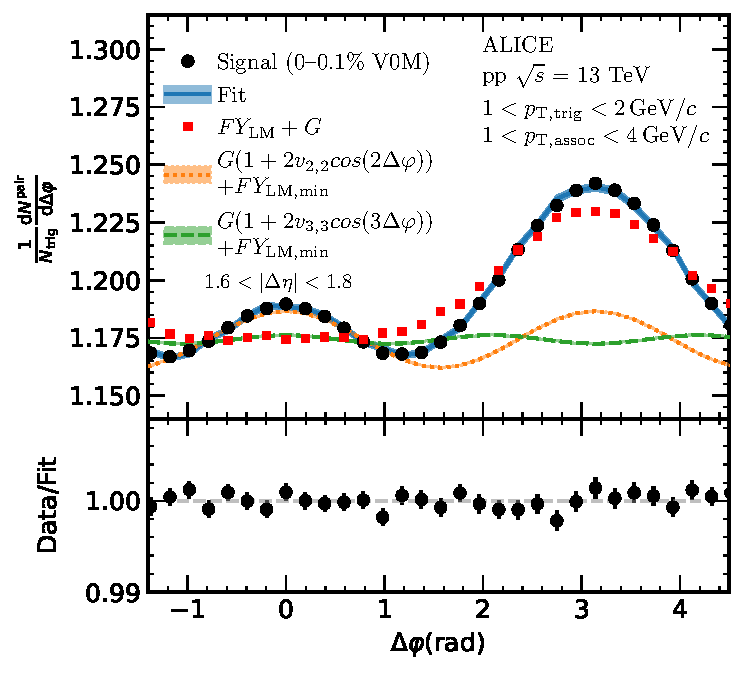
\includegraphics[width=0.6\textwidth]{figures/Fig1_FlowExt.pdf} 
	\caption{The template fit results with the low-multiplicity templates. The black markers show the signal for the 0--0.1\% multiplicity percentile and its fit as a blue band. The red squares correspond to the low-multiplicity signal. The orange and green curves correspond to the extracted $v_2$ and $v_3$ signals, respectively. The $\chi^{2}$ divided by the number of degrees of freedom is 0.894}
	\label{fig:flowext}
\end{figure}

Figure~\ref{fig:flowext} shows the template fit results for 0--0.1\% multiplicity percentile pp collisions at $\sqrt{s}$ = 13 TeV. The low-multiplicity yield,  $Y_{\rm{LM}}(\Delta\varphi)$, is shown in red squares, and the extracted $v_{2}$ and $v_{3}$ as orange and green respectively. The results on the scale factor $F$ in different multiplicity percentiles and systems are summarized in Tab.~\ref{tab:FpppPb}. 
In pp collisions, they are larger at high multiplicity, and in p--Pb collisions they are closer to unity at low multiplicity. This suggests that the jet fragmentation yield on the away-side increases with multiplicity, which is more pronounced in pp collisions.
 In previous ALICE results~\cite{ALICE:2012eyl,ALICE:2013snk}, it was assumed that the jet contribution is unchanged as a function of multiplicity (i.e. $F$ was assumed to be 1), which may lead to an underestimation of non-flow contamination in the final measurements of anisotropic flow. 
 The fit to the signal, Eq.~\ref{eq:narray}, is shown as a blue band, and the signal-to-fit ratio is shown in the bottom panel. 
%let's add chiq value of the fit
\begin{table}[h!]
\caption{The scale factor $F$ for various multiplicity percentiles in pp (top) and p--pPb (bottom) collisions.}
\begin{tabular}{|c|c|c|c|c|c}
\hline
V0M (pp)& 0--0.1\% & 1--5\% & 5--20\% & 20--60\% \\
\hline
$F$ & 1.504$\pm$0.017 & 1.414$\pm$0.030 & 1.360$\pm$0.019 & 1.208$\pm$0.015 \\
\hline
\end{tabular}
\centering
\resizebox{\textwidth}{!}{%
\begin{tabular}{|c|c|c|c|c|c|c|}
\hline
V0A (p--pPb)& 0--5\% & 5--10\% & 10--20\% & 0--20\% & 20--40\% & 40--60\% \\
\hline
$F$& 1.135$\pm$0.026 & 1.140$\pm$0.026 & 1.152$\pm$0.021 & 1.145$\pm$0.017 &1.092$\pm$0.015 & 1.083$\pm$0.015 \\
\hline
\end{tabular}
}
\label{tab:FpppPb}
\end{table}

In the following, the near and away-side jet fragmentation yields are calculated to verify the template fit method by comparing the jet fragmentation yields to the PYTHIA model.
The near-side jet-like yields are extracted from the near-side $\Delta\eta$ correlations, defined in $|\Delta\varphi|<$~1.3 as the following
\begin{eqnarray}
Y^{near}_{\rm{frag}} = \int_{|\Delta \eta|<1.3} \left( \frac{1}{\it{N}_{\rm{trig}}} \frac{ \rm{d}\it{}N_{\rm{pair}} }{ \rm{d}\Delta\eta } \right) \rm{d} \Delta\eta \quad.
\label{eq:Ynear}
\end{eqnarray}
%The range of $\Delta\varphi$ is chosen to be 1.3 in order for the projection range to fully cover the near-side peak in $\Delta\varphi$. 
%The correlations in the same jet mainly contribute to $(\Delta\eta, \Delta\varphi) \sim (0,0)$ due to the similar outgoing direction of particles inside the jet along the jet axis. 
As can be seen in Eq.~\ref{eq:Ynear}, the yield of the jet fragmentation is calculated by integrating the $\Delta\eta$ correlation over $|\Delta\eta|<1.3$ after applying the ZYAM procedure~\cite{Ajitanand:2005jj} because the flow coefficients have a weak dependence on $\eta$~\cite{ATLAS:2011ah,PHENIX:2018hho,ALICE:2016tlx}. The ZYAM procedure is applied by finding the minimum value of $\Delta\eta$ correlations within $|\Delta\eta|<1.3$, which results in pointing the minimum position to be $|\Delta\varphi|=1.3$.

The away-side jet-like yield in data is calculated from the low-multiplicity template fit method as $Y^{\rm{away, HM}}_{\mathrm{frag}} = Y^{\rm{away, LM}}_{\mathrm{frag}} \times F$, where $F$ is the parameter from Eq.~\ref{eq:narray}. The $Y^{\rm{away, LM}}_{\mathrm{frag}}$ is directly obtained by integrating the away-side low-multiplicity $\Delta\varphi$ correlation function in the low-multiplicity sample over $\pi/2 < \Delta\varphi < 3\pi/2$.
In PYTHIA, it is possible to directly measure  $Y^{\rm{away}}$ from the $\Delta\varphi$ correlation functions since the model does not include any flow contributions.

\begin{figure}[h!]
	\centering
	\hspace{-3em}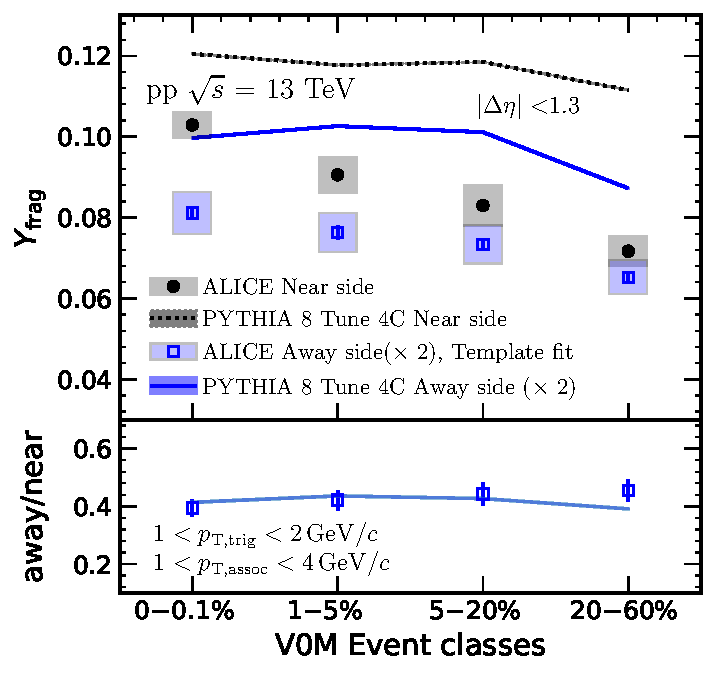
\includegraphics[width=0.6\textwidth]{figures/Fig5_Plot_v2Mult.pdf} 
	\caption{The $Y^{\rm{frag}}$ for the near- and away-side as a function of multiplicity percentiles with both ALICE and PYTHIA data. The ratio includes the combined statistical and systematic errors in quadrature.}
	\label{fig:Ymult}
\end{figure}

Figure~\ref{fig:Ymult} presents the $Y^{\mathrm{near}}_{\rm{frag}}$ and $Y^{\mathrm{away}}_{\rm{frag}}$, for both ALICE data and PYTHIA 8 Tune 4C as a function of multiplicity percentile in pp collisions at $\sqrt{s}=13$ TeV. The transverse momentum range for trigger particles is $1<p_\mathrm{T,trig}<2$ GeV/c and for associated particles $1<p_\mathrm{T,assoc}<4$ GeV/c. ALICE data points are shown as circle and square markers, whereas PYTHIA is shown as lines. The near-side yields are shown in black, and the away-side yields in blue.
The near- to away-side ratio for ALICE and PYTHIA data is shown in the bottom panel. While PYTHIA overestimates ALICE data for both $Y^{\mathrm{near}}_{\rm{frag}}$ and $Y^{\mathrm{away}}_{\rm{frag}}$, the ratio to PYTHIA is consistent with the ALICE data in the multiplicity percentiles studied. This ratio can be explained by the pair acceptance effect caused by the limited ALICE $\eta$ acceptance~\cite{PHENIX:2006gto}, which implies that the enhanced jet fragmentation yields in away-side in high-multiplicity events with respect to low-multiplicity events~\cite{ALICE:2013tla,ALICE:2014mas} are taken into account in by the low-multiplicity template method. In summary, the difference between the near-side and away-side jet fragmentation yields in PYTHIA is solely caused by the jet acceptance effects of the two-particle correlation functions. This ratio in data where the away-side jet fragmentation yields are measured with the low-multiplicity template agrees well with PYTHIA as well as the calculations in Ref.~\cite{PHENIX:2006gto}, which provides only the jet acceptance effect.
%It is worthwhile to noting that, even though this method measures the jet yields on the away side from the fit, these yields were not reported in previous measurements~\cite{}.

%\begin{figure}[h!]
%		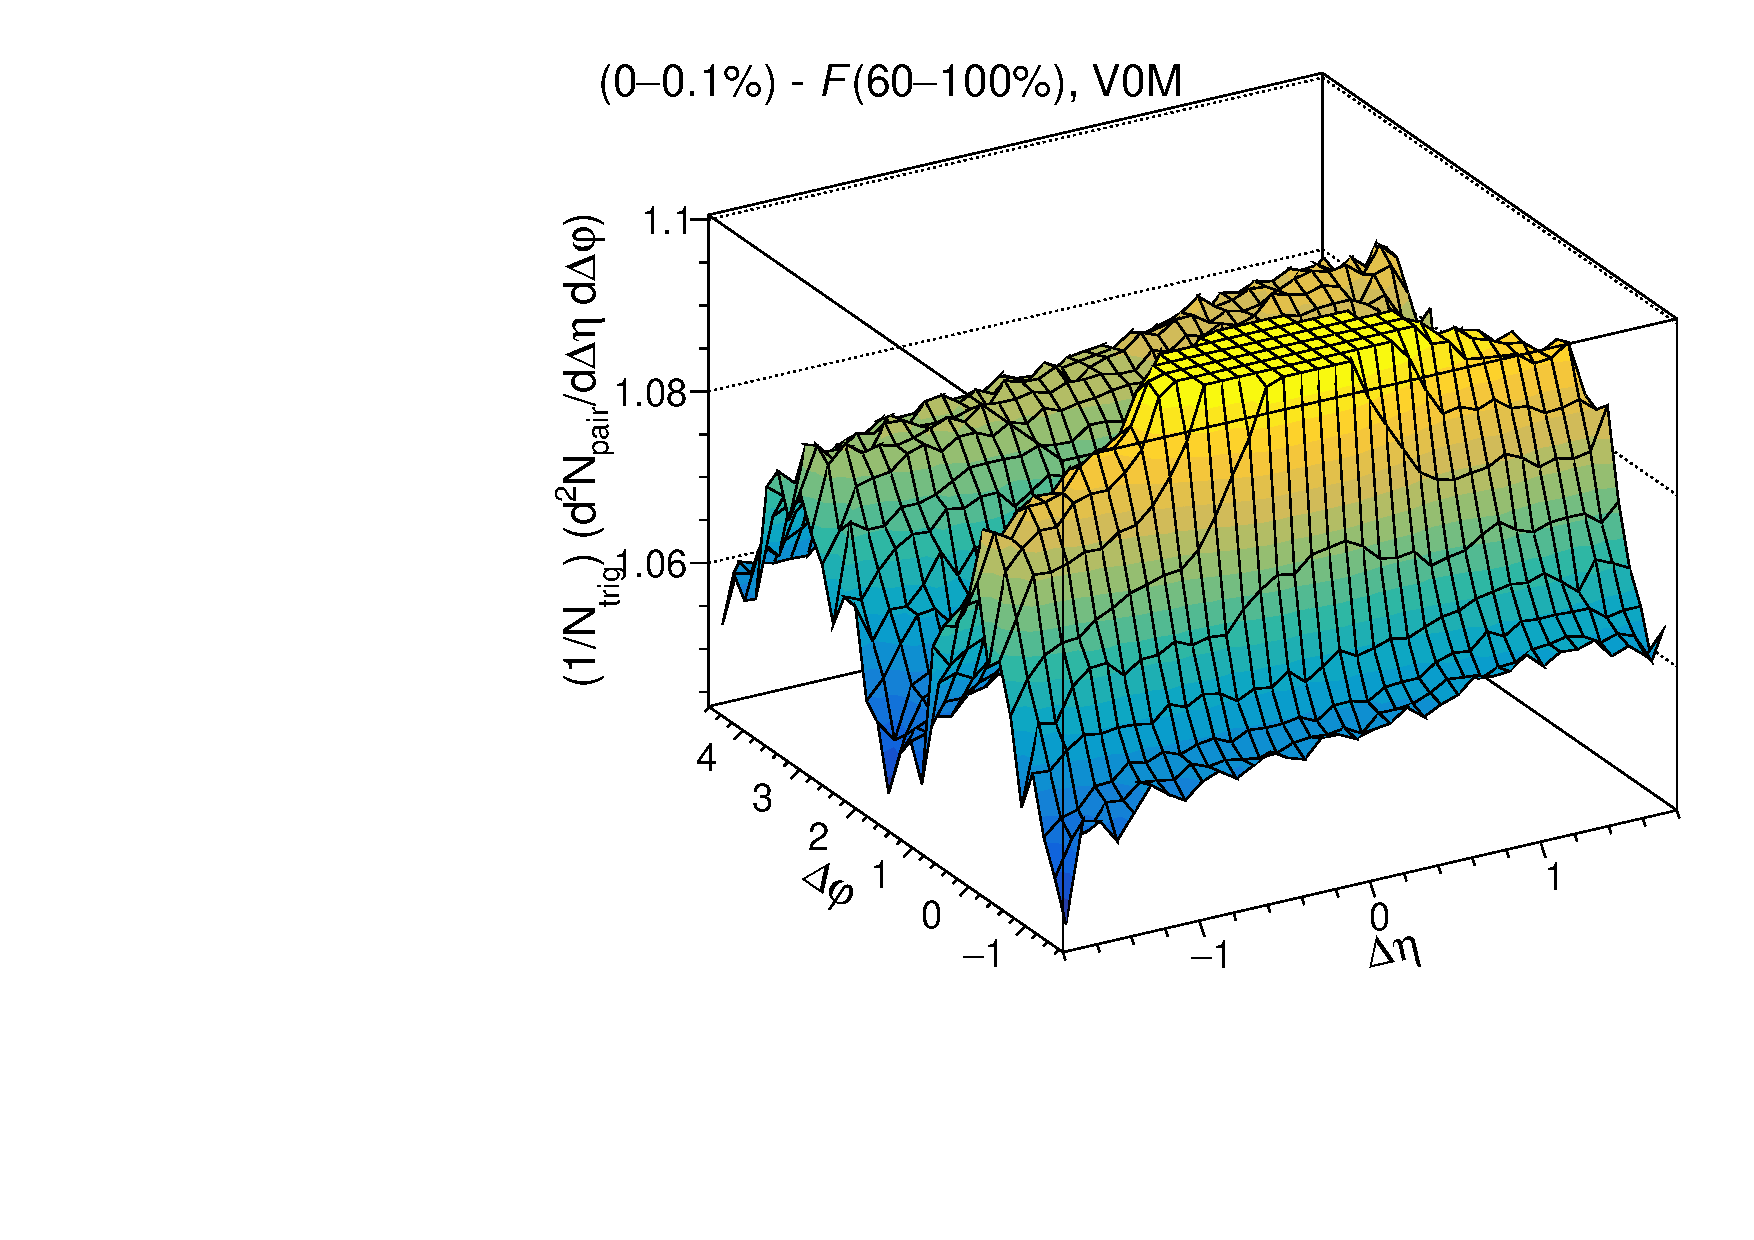
\includegraphics[width=0.5 \textwidth]{figures/Fig1_ppSub.pdf}
%  		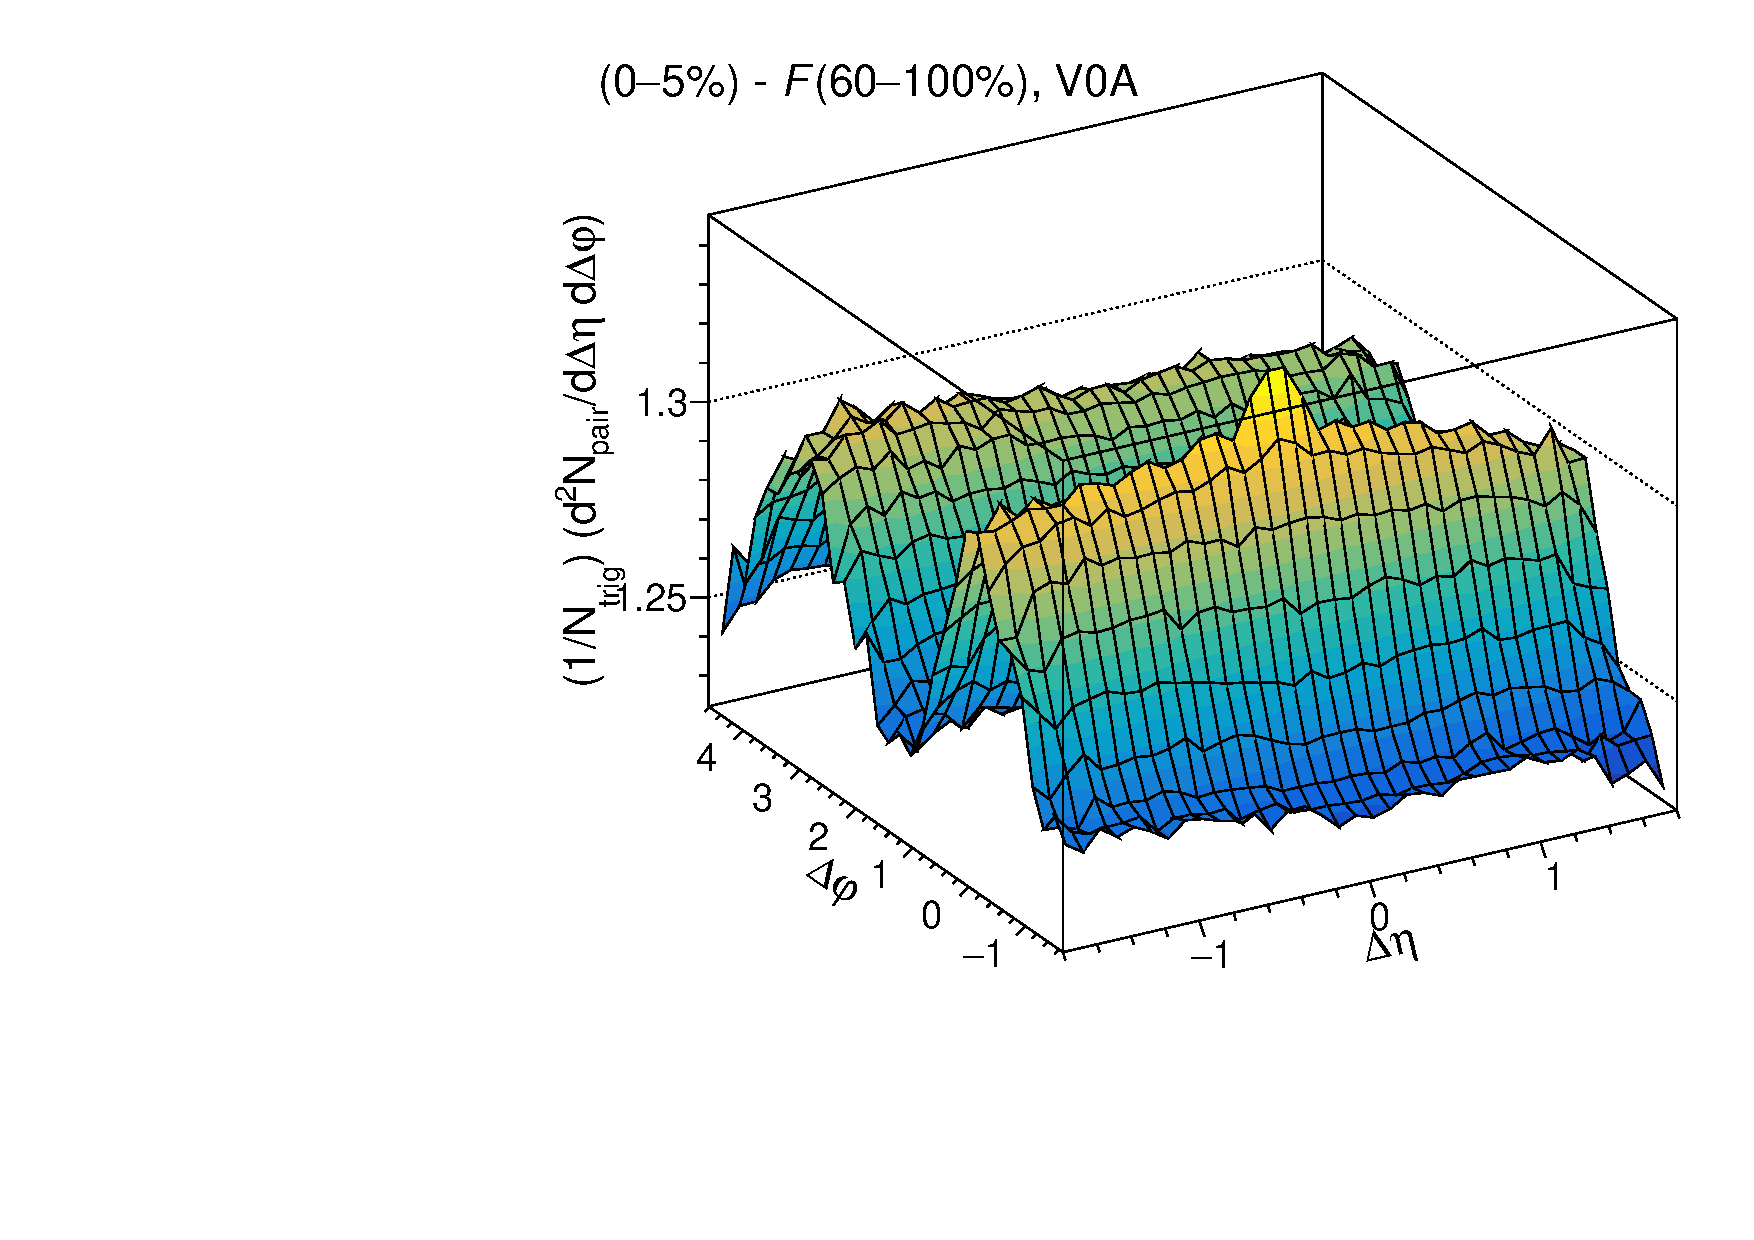
\includegraphics[width=0.5 \textwidth]{figures/Fig1_pPbSub.pdf}
%\caption{The subtracted one as (0--0.1)\%-$F$(60--100\%) is shown on the right. The subtracted one as (0--5)\%-$F$(60--100\%) is shown on the right. Note that the near-side jet peaks exceed the chosen range of the $z$-axis. The intervals of $\pttrig$ and $\ptassoc$ are 1~$<\it{p}_{\rm{T}}<$~2~GeV/$c$ in all cases.}
%\label{fig:doubleridge_sub}
%\end{figure}

%The subtracted one as (0--5)\%-$F$(60--100\%) on the right. Similarly, the ones in p--Pb collisions at $\sqrt{s_{\mathrm{NN}}}=5.02$ TeV are shown in Fig.~\ref{fig:doubleridge_sub}. The $F$ values can be found in Tables~\ref{tab:Fpp} and \ref{tab:Fpb}, which come from the low-multiplicity template fit in a given multiplicity percentile as described in Sec.~\ref{sec:ana}. 
%show an asymmetry in delta eta, e.g. in pp collisions the signal
%rises going from negative to positive delta eta values

The flow coefficients, $v_{n}$ of the trigger particles, can be extracted from the template fit with the use of the observed factorization of $v_{n,n}$ coefficients to single harmonics~\cite{ATLAS:2015hzw,ATLAS:2016yzd} by using
\begin{eqnarray}
v_{n}(p_{\rm{T,trig}}) = v_{n,n}(p_{\rm{T,trig}}, p_{\rm{T,assoc}}) / \sqrt{ v_{n,n}(p_{\rm{T,assoc}},p_{\rm{T,assoc}})},
\end{eqnarray}
where $v_{n,n}(p_{\rm{T,assoc}}$ and $p_{\rm{T,assoc}})$ are measured in 1~$<p_{\rm{T,trig}}<$~4~GeV/$c$ interval as the $p_{\rm{T,assoc}}$ range is fixed with 1~$<p_{\rm{T,assoc}}<$~4~GeV/$c$. In the following sections, unless explicitly stated otherwise, $v_n$ will refer to $v_n(p_{\rm{T,trig}})$.
Different event scale selections are investigated by selecting events that include a hard jet or a high-$\pt$ leading particle within the mid-rapidity region, it is possible to study the impact parameter dependence of flow coefficients in pp collisions~\cite{Sjostrand:1986ep,Frankfurt:2010ea}. This event scale is set by requiring a minimum $\pt$ of the leading track ($\ptlead$) or the reconstructed jet ($\ptjet$) at midrapidity. The leading particle track requires to be within $|\eta|<0.9$ and $0<\phi<2\pi$, and the jets are reconstructed with the anti-$k_{\rm{T}}$ algorithm~\cite{Cacciari:2008gp,Cacciari:2011ma}, with $R=0.4$ for only charged particles. This analysis uses the $\pt$ scheme as the recombination scheme. In the same way, as for the leading particle tracks, the jets are selected in the full azimuthal angle ($0<\phi<2\pi$) but in an $\eta$-range of $|\eta_\mathrm{jet}|<0.4$. The $\pt$ of jets $\ptjet$ is corrected for the underlying event density that is measured using the $k_{\rm{T}}$ algorithm with $R=$~0.2~\cite{Acharya:2018eat}.

%%%%%%%%%%%%%%%%%%%%%%%%%%%%%%%%%%%%%%%%%%%%%%%%%%%%%%%%%%

\section{Systematic uncertainties}
\label{sec:uncertainties}

\begin{table}[h!]
\caption{The relative systematic uncertainties of $Y^{\rm{near}}$, $Y^{\rm{away,LM}}$, $F$, $v_{2}$, and $v_{3}$. Numbers given in ranges correspond to minimum and maximum uncertainties. ``negl." is assigned if the systematic deviation is contaminated by the statistical fluctuation. ``N.A" is assigned when the systematic variation is not relevant to the measurement. }
\centering
\label{tab:syst}
\resizebox{\textwidth}{!} {
\begin{tabular}{c|ccccccc}
\hline 
\multirow{3}{*}{Sources}  & \multicolumn{7}{c}{Systematic uncertainty (\%)} \\ \cline{2-8} 
& \multirow{2}{*}{$Y^{\rm{near}}$} & \multirow{2}{*}{$Y^{\rm{away,LM}}$} & \multirow{2}{*}{$F$} & \multicolumn{2}{c}{$v_{2}$} & \multicolumn{2}{c}{$v_{3}$}  \\   \cline{5-8}
& & & & pp & p--Pb & pp & p--Pb  \\ \cline{1-8} 
Primary vertex       & $\pm$0.2--0.5 & $\pm$0.1      & $\pm$1.0--2.5 & $\pm$0.2--1.8 & $\pm$0.8 & $\pm$1.4 & $\pm$3.9 \\ 
Pileup rejection     & $\pm$0.1--0.5 & $\pm$0.2      & $\pm$0.4--1.5 & negl.         & $\pm$0.6 & negl. & $\pm$1.4 \\ 
Tracking		     & $\pm$1.0--3.0 & $\pm$2.0      & $\pm$0.6--2.4 & $\pm$0.2--3.0 & negl. & $\pm$5.0--6.9 & negl. \\ 
Event mixing	     & $\pm$0.2--0.7 & $\pm$0.2--0.5 & $\pm$0.0--3.3 & $\pm$0.3--4.6 & $\pm$0.8 & $\pm$2.8--3.1 & $\pm$0.8 \\ 
Low mult. definition & N.A.          & $\pm$0.5--3.5 & $\pm$0.7--6.0 & negl.         & $\pm$1.9 & negl. & $\pm$9.2\\ 
ITS-TPC matching 	 & $\pm$2.0--3.0 & $\pm$2.0--3.0 & N.A.          & N.A.          & N.A. & N.A. & N.A\\ 
Efficiency correction& $\pm$1.0--4.4 & $\pm$1.0--4.4 & N.A.          & N.A.          & N.A. & N.A. & N.A\\ 
$\eta$ gap range   	 & N.A.          & N.A.          & $\pm$0.1--3.2 & $\pm$1.0--5.0 & $\pm$0.4 & negl. & negl. \\ 

\hline 
Total (in quadrature)& $\pm$2.5--6.1 & $\pm$5.0--5.5 & $\pm$1.8--7.1 & $\pm$0.8--5.7 & $\pm$2.3 & $\pm$6.1--7.5 & $\pm$10.1 \\ 
\hline 
\end{tabular}
}
\end{table}

The systematic uncertainties of $Y^{\rm{near}}$, $Y^{\rm{away,LM}}$, and $F$ are estimated by varying the analysis selection criteria and corrections in pp collisions, while the systematic uncertainties of $v_{2}$ and $v_{3}$ are estimated in pp and p--Pb collisions. All systematic uncertainties are summarized in Table~\ref{tab:syst}.

The uncertainty associated to the selected range of the primary vertex is estimated by varying the accepted range from $|z_\mathrm{vtx}|<$~8~cm to $|z_\mathrm{vtx}|<$~6~cm. The variation of the range allows testing detector acceptance effects on the measurement. The estimated uncertainties of $Y^{\rm{near}}$ and $Y^{\rm{away,LM}}$ are 0.2--0.5\% and 0.1\%, respectively. The uncertainties associated with the primary vertex selection are estimated to be 1.0--2.5\%, 0.2--1.8\%, and 1.4--3.9\% for $F$, $v_{2}$, and $v_{3}$, respectively. 

Another source of systematic uncertainty is related to pileup rejection. Pileup events are rejected with different rejection criteria, such as the number of track contributors required for the reconstruction of pileup event vertices, where the number is changed from the default value of 3 to 5. The uncertainties of $Y^{\rm{near}}$ and $Y^{\rm{away,LM}}$ are estimated to be 0.1--0.5\% and 0.2\%, respectively. The estimated uncertainties are negligible for $F$. The estimated uncertainties of $v_{2}$ and $v_{3}$ are 0.6\% and 1.4\%, respectively.

The systematic uncertainty from the track selection criteria is estimated by employing the other track selection criteria so called “global tracks”, which is described in Ref~\cite{ALICE:2021ptz}. The global track is required to have two hits in the ITS (at least one in the SPD) and at least 70 clusters in TPC. Due to inefficient parts of the SPD, the azimuthal distribution of global tracks is not uniform, which can be corrected within the azimuthal interval we defined including different $p_{\mathrm{T}}$ inefficiency of this tracking. The systematic uncertainty from the different track selection criteria is  0.2--3.0\% for $v_{2}$ and  5.0--6.9\% for $v_{3}$. 


An additional systematic uncertainty from the event-mixing is estimated by varying the interval of the primary vertex range, where events are mixed. The default value of 2~cm is changed to 1~cm. The resulting uncertainty of jet fragmentation yield ($Y^{\rm{near}}$ and $Y^{\rm{away,LM}}$) is 0.2--0.7\%. The uncertainties of $F$, $v_{2}$, and $v_{3}$ are estimated to be 0.3--4.6\%.

The systematic uncertainty from the low-multiplicity definition is estimated by changing the range of the low-multiplicity centrality percentile. There is no universal definition for the low-multiplicity, and the default range for the low-multiplicity in the present paper is set to 60--100\%, and changed to 70--100\%. The uncertainty of $Y^{\rm{away,LM}}$ is estimated to be 0.5--3.5\%. Note that the measurement of $Y^{\rm{near}}$ is not relevant to the low-multiplicity definition, and the uncertainty is not estimated. The uncertainties of $F$, $v_{2}$, and $v_{3}$ are estimated to be 0.7--9.2\%.

The systematic uncertainty from matching the track reconstructed by the TPC and the corresponding signal in the ITS is estimated by evaluating the fraction of the mismatch between them. The estimated uncertainties of $Y^{\rm{near}}$ and $Y^{\rm{away,LM}}$ are 2.0--3.0\%.

The systematic uncertainty from the efficiency correction for unidentified charged particles is estimated by comparing two correlation functions. One is constructed using true information in MC samples. The other is constructed using the reconstructed tracks, where reconstructed tracks are corrected for the tracking efficiency. The estimated uncertainty is 0.1--5.0\%.

Due to the limited $\eta$ acceptance of the TPC, non-flow contributions mainly originating from jet fragmentations affect the flow measurement. As the shape of short-range correlations mostly attributed to jets is getting broader with the decreasing $\pt$, the systematic uncertainty from $\eta$-acceptance significantly depends on the $p_{\rm{T}}$. To estimate the related uncertainty, the minimum $\Delta\eta$ gap is changed from 1.6 to 1.7 for constructing long-range $\Delta\varphi$ correlations.  The estimated uncertainties of $F$, $v_{2}$, and $v_{3}$ are 0.1--5.0\%.





